% !TEX program = xelatex
\documentclass[11pt,a4paper]{article}
\usepackage{fontspec}
\setmainfont{Calibri}
\setmonofont[Scale=0.88]{Consolas}
\newfontfamily\symbolfont{Segoe UI Symbol}
\usepackage{polyglossia}\setdefaultlanguage{polish}
\usepackage[table]{xcolor}
\usepackage{booktabs,longtable,array,geometry,enumitem,graphicx,fancyhdr,caption}
\usepackage[most]{tcolorbox}
\PassOptionsToPackage{hyphens}{url}
\usepackage[hidelinks,unicode]{hyperref}
\emergencystretch=2.5em
\geometry{a4paper,margin=2.1cm,top=2.3cm,bottom=2.3cm}
\setlength{\parindent}{0pt}\setlength{\parskip}{5pt}
\definecolor{apteal}{HTML}{0E7C86}
\definecolor{apteallight}{HTML}{E6F4F5}
\definecolor{apgrey}{HTML}{F3F4F6}
\definecolor{apamber}{HTML}{B45309}
\definecolor{apamberlight}{HTML}{FEF3C7}
\definecolor{apred}{HTML}{B91C1C}
\definecolor{apredlight}{HTML}{FEE2E2}
\definecolor{apgreen}{HTML}{15803D}
\definecolor{apgreenlight}{HTML}{DCFCE7}
\renewcommand{\arraystretch}{1.25}
\captionsetup{font=small,labelfont=bf}
\pagestyle{fancy}\fancyhf{}
\fancyfoot[L]{\small AMPERE POINT — OCPP dla Q11: strony i rozwiązania · v1 · 2026-09-27}
\fancyfoot[R]{\small\thepage}
\renewcommand{\headrulewidth}{0pt}
\newtcolorbox{uwaga}[1][Uwaga]{enhanced,breakable,colback=apamberlight,colframe=apamber,title={#1},fonttitle=\bfseries,boxrule=0.6pt,arc=2pt,left=6pt,right=6pt,top=4pt,bottom=4pt}
\newtcolorbox{info}[1][Jak to działa]{enhanced,breakable,colback=apteallight,colframe=apteal,title={#1},fonttitle=\bfseries,boxrule=0.6pt,arc=2pt,left=6pt,right=6pt,top=4pt,bottom=4pt}
\newtcolorbox{wazne}[1][Ważne]{enhanced,breakable,colback=apredlight,colframe=apred,title={#1},fonttitle=\bfseries,boxrule=0.6pt,arc=2pt,left=6pt,right=6pt,top=4pt,bottom=4pt}
\newtcolorbox{przyklad}[1][Przykład liczbowy]{enhanced,breakable,colback=apgreenlight,colframe=apgreen,title={#1},fonttitle=\bfseries,boxrule=0.6pt,arc=2pt,left=6pt,right=6pt,top=4pt,bottom=4pt}
\newtcolorbox{kodbox}{enhanced,breakable,colback=apgrey,colframe=apgrey,boxrule=0pt,arc=2pt,left=5pt,right=5pt,top=3pt,bottom=3pt,fontupper=\ttfamily\footnotesize}
\setlist{nosep,leftmargin=*}
\setcounter{secnumdepth}{2}
\begin{document}

{\LARGE\bfseries OCPP dla Q11: kto jest kim i cztery sposoby podłączenia\par}
{\large Strony, schematy i porównanie z testem na DevKicie · AMPERE POINT · 27 września 2026 · oprac. Dawid Cekała\par}
\vspace{4pt}\textcolor{apteal}{\rule{\textwidth}{1.2pt}}

\section*{W skrócie}

\begin{itemize}
\item OCPP to język, którym ładowarka rozmawia z serwerem operatora, czyli firmy rozliczającej ładowanie. Ładowarka sama łączy się z tym serwerem i utrzymuje połączenie przez cały czas.
\item Q11 nie zna OCPP. Potrzebny jest tłumacz, który z jednej strony mówi OCPP, a z drugiej ustawia pola modułu Shelly. W teście 25.09 tłumaczem był most, czyli program \texttt{most\_q11.py} na laptopie.
\item Cztery rozwiązania różnią się tylko miejscem, w którym działa tłumacz: w systemie modułu X1, w naszym skrypcie w X1, na serwerze AmperePoint albo na małym komputerze u klienta.
\item Część między sterownikiem Q11 a modułem, czyli protokół Tuya i nasz skrypt usługi, jest we wszystkich rozwiązaniach taka sama. Działa już dziś.
\item Rekomendacja: rozwiązanie 3 od razu, a Shelly zapytać o rozwiązanie 1. Uzasadnienie w rozdziale „Rekomendacja”.
\end{itemize}

\section{Strony: kto jest kim}

\begin{figure}[h]\centering
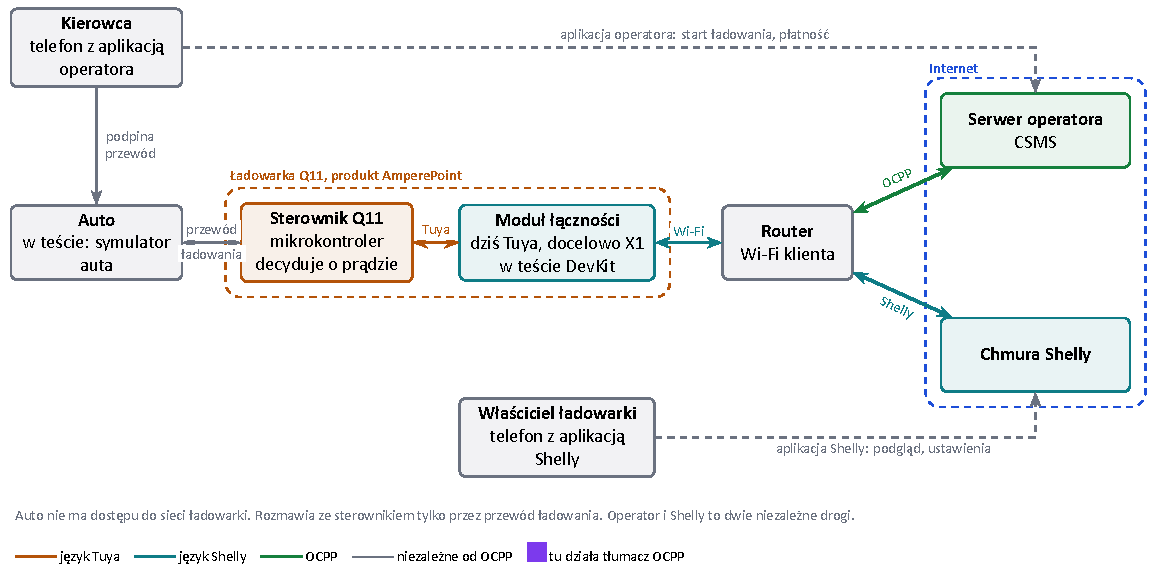
\includegraphics[width=1.00\textwidth]{img/ocpp_strony.pdf}
\caption{Wszystkie strony wokół ładowarki. Droga do operatora (zielona) i droga do Shelly (turkusowa) są od siebie niezależne.}
\end{figure}

\begin{longtable}{>{\raggedright\arraybackslash}p{3.00cm}>{\raggedright\arraybackslash}p{9.52cm}>{\raggedright\arraybackslash}p{2.76cm}}
\toprule
\rowcolor{apteallight}\textbf{Strona} & \textbf{Czym jest} & \textbf{W teście 25.09} \\
\midrule\endhead
\bottomrule\endfoot
Kierowca & Osoba, która ładuje auto. Ładowanie zaczyna w aplikacji operatora albo kartą. & my, polecenie \texttt{start} w pliku \texttt{polecenia.\allowbreak{}txt} \\
Auto & Pobiera prąd. Ze sterownikiem ładowarki rozmawia tylko przez przewód ładowania, sygnałem pilota. Do sieci ładowarki nie ma dostępu. & symulator auta \\
Sterownik Q11 & Mikrokontroler na płytce ładowarki. Włącza i wyłącza prąd, mierzy, pilnuje bezpieczeństwa. Nie ma Wi-Fi. & płytka Q11 w biurze \\
Moduł łączności & Mała płytka z Wi-Fi w obudowie Q11. Dziś Tuya WBR3, docelowo Shelly X1. & DevKit, \texttt{192.\allowbreak{}168.\allowbreak{}0.\allowbreak{}238} \\
Router klienta & Łączy moduł z internetem. Przepuszcza połączenia wychodzące, blokuje przychodzące. & router biura \\
Operator & Firma, która prowadzi ładowanie jako usługę: wydaje karty, nalicza opłaty, widzi stan ładowarek, zdalnie uruchamia i ogranicza ładowanie. Po angielsku Charge Point Operator. & rolę grał serwer testowy \\
Serwer operatora, CSMS & Program operatora, z którym łączą się ładowarki. Nazwa od Charging Station Management System. Operator może mieć własny albo wynająć gotowy, np. Monta lub Virta. & \texttt{csms\_test.py} na laptopie, port 9000 \\
Tłumacz OCPP & Program, który mówi OCPP do operatora i ustawia pola modułu. Nazywany też mostem albo bramką. & \texttt{most\_q11.py} na laptopie \\
Chmura i aplikacja Shelly & Serwery Shelly i aplikacja w telefonie właściciela. Podgląd i ustawienia, bez rozliczeń. Działa niezależnie od OCPP. & wyłączona \\
Właściciel ładowarki & Ten, kto kupił Q11. W domu to zwykle ta sama osoba co kierowca, na parkingu firma. & biuro \\
AmperePoint & Producent Q11. Ustala produkt w portalu Shelly X i pisze skrypt usługi. W rozwiązaniu 3 prowadzi też serwer z tłumaczem. & my \\
Shelly & Producent modułu X1 i jego systemu. Tylko Shelly może zmienić system w module. & brak udziału \\
Instalator & Montuje ładowarkę u klienta i wpisuje ustawienia, w tym adres operatora. & my \\
\end{longtable}

\subsection{Kiedy w ogóle potrzebny jest operator}

Operator jest potrzebny wtedy, gdy za prąd płaci ktoś inny niż kierowca albo gdy ktoś musi ładowanie rozliczyć. Przykłady:


\begin{itemize}
\item firma z samochodami służbowymi, która zwraca pracownikom koszt ładowania w domu,
\item hotel lub parking, który sprzedaje ładowanie gościom,
\item sieć publicznych ładowarek.
\end{itemize}

Przykład liczbowy: pracownik ładuje służbowe auto w domu, 300 kWh w miesiącu. Przy cenie 1,20 zł za kWh firma zwraca mu 360 zł. Żeby to policzyć, operator dostaje z ładowarki stan licznika energii na początku i na końcu każdej sesji.


W domu, gdzie kierowca płaci własny rachunek za prąd, OCPP zwykle nie jest potrzebne. Wystarczy aplikacja.


\section{OCPP w jednym akapicie}

Ładowarka jest klientem, serwer operatora jest serwerem. Ładowarka otwiera jedno stałe połączenie pod adres operatora z dopisanym swoim identyfikatorem, np. \texttt{wss:\allowbreak{}/\allowbreak{}/\allowbreak{}csms.\allowbreak{}przyklad-\allowbreak{}operatora.\allowbreak{}pl/\allowbreak{}ocpp/\allowbreak{}Q11-\allowbreak{}543204516334}. Połączenie zaczyna zawsze ładowarka, bo stoi za routerem klienta, a router nie wpuszcza połączeń z internetu. Gdy połączenie już jest, działa w obie strony.


To stałe połączenie to WebSocket. Działa jak rozmowa telefoniczna, która trwa cały czas: każda strona może się odezwać w dowolnej chwili. Zwykłe zapytanie HTTP działa jak list z odpowiedzią: zaczyna zawsze pytający. OCPP potrzebuje telefonu, bo operator musi móc w każdej chwili powiedzieć „ogranicz do 10 A” albo „zacznij ładowanie”.


\section{Część wspólna wszystkich rozwiązań}

Sterownik Q11 i moduł rozmawiają protokołem Tuya przez przewód. Nasz skrypt usługi w module zamienia punkty danych Tuya na pola Shelly i z powrotem. Na przykład limit prądu to w Q11 punkt danych 4, a w module pole limitu prądu.


Ta część jest sprawdzona. Limit 10 A i 12 A ustawiony przez MQTT i przez OCPP Q11 potwierdziła swoim meldunkiem. Każde z czterech rozwiązań korzysta z niej bez zmian. Rozwiązania różnią się tylko tym, kto ustawia pola i skąd.


\section{Punkt odniesienia: test na DevKicie}

\begin{figure}[h]\centering
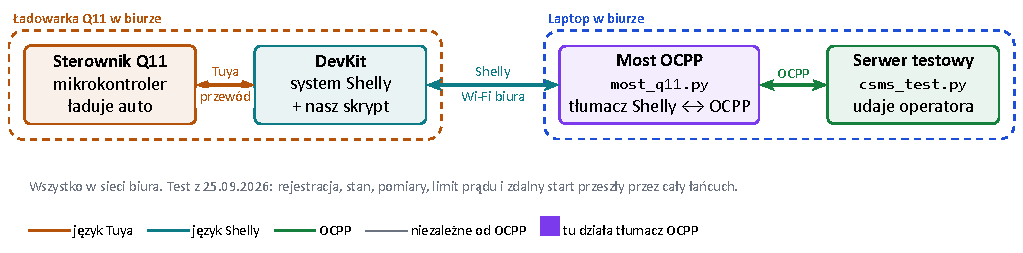
\includegraphics[width=1.00\textwidth]{img/ocpp_rozw_0_test.pdf}
\caption{Test z 25.09.2026. Tłumacz i serwer testowy działały na laptopie w biurze.}
\end{figure}

Przykład: operator ogranicza ładowanie do 10 A.


\begin{enumerate}
\item Serwer testowy wysyła polecenie OCPP \texttt{SetChargingProfile} z limitem 6900 W.
\item Most na laptopie przelicza waty na ampery: 6900 W podzielone przez 690 daje 10 A. Liczba 690 to trzy fazy razy 230 V.
\item Most wysyła do DevKitu przez Wi-Fi polecenie w języku Shelly: ustaw pole limitu prądu na 10.
\item Nasz skrypt w DevKicie układa ramkę Tuya \texttt{55 AA 00 06 00 08 04 02 00 04 00 00 00 0A 21} i wysyła ją do sterownika.
\item Sterownik najpierw odsyła starą wartość, a po około sekundzie nową, 10 A.
\end{enumerate}

U klienta tak zostać nie może. Laptop musiałby działać cały czas i stać w tej samej sieci co ładowarka. Każde z rozwiązań poniżej usuwa laptop w inny sposób.


\clearpage
\section{Rozwiązanie 1: OCPP w systemie modułu X1, pisze Shelly}

\begin{figure}[h]\centering
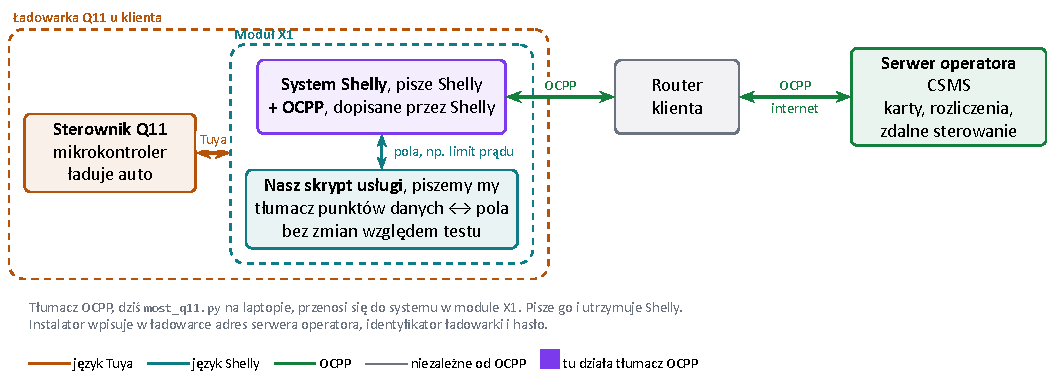
\includegraphics[width=1.00\textwidth]{img/ocpp_rozw_1_w_x1.pdf}
\caption{Rozwiązanie 1. Tłumacz przenosi się z laptopa do systemu modułu X1.}
\end{figure}

\subsection{Jak to działa względem testu}

W teście tłumaczem był most na laptopie. W rozwiązaniu 1 Shelly dopisuje taki sam tłumacz do systemu modułu. Laptop znika, a moduł sam łączy się z operatorem przez router klienta.


\begin{longtable}{>{\raggedright\arraybackslash}p{6.12cm}>{\raggedright\arraybackslash}p{4.33cm}>{\raggedright\arraybackslash}p{4.83cm}}
\toprule
\rowcolor{apteallight}\textbf{Krok} & \textbf{Test na DevKicie} & \textbf{Rozwiązanie 1} \\
\midrule\endhead
\bottomrule\endfoot
Kto otwiera połączenie z operatorem & most na laptopie & moduł X1 \\
Skąd bierze adres operatora & wpisany w programie mostu & z ustawień modułu \\
Kto przelicza 6900 W na 10 A & most & kod OCPP w systemie X1 \\
Kto ustawia pole limitu prądu & most, poleceniem przez Wi-Fi & kod OCPP w systemie X1, wewnątrz modułu \\
Kto układa ramkę Tuya & nasz skrypt & nasz skrypt, bez zmian \\
Kto zgłasza operatorowi stan „ładuje” & most, po odczycie pola stanu & kod OCPP w systemie X1 \\
\end{longtable}

\subsection{Gdzie wpisuje się adres operatora}

Tak by to prawdopodobnie wyglądało. Szczegóły ustala Shelly.


\begin{itemize}
\item \textbf{W portalu Shelly X, raz dla wszystkich Q11:} włączenie OCPP i opis, które pole jest limitem prądu, stanem, licznikiem energii. Dziś tę pracę wykonuje most w swoich funkcjach.
\item \textbf{W każdej ładowarce osobno:} adres serwera operatora, identyfikator ładowarki i hasło. Każdy klient może mieć innego operatora, więc tego nie da się wpisać w portalu raz dla wszystkich. Wpisuje instalator na stronie modułu albo w aplikacji.
\end{itemize}

\subsection{Co musi zrobić Shelly i czy starczy pamięci}

Shelly musi dopisać do systemu klienta OCPP 1.6J z szyfrowaniem TLS i hasłem, ustawienia dla instalatora i powiązanie z polami. My dostarczamy opis pól.


\begin{longtable}{>{\raggedright\arraybackslash}p{3.00cm}>{\raggedright\arraybackslash}p{1.71cm}>{\raggedright\arraybackslash}p{5.00cm}>{\raggedright\arraybackslash}p{5.13cm}}
\toprule
\rowcolor{apteallight}\textbf{Zasób X1} & \textbf{Wolne dziś} & \textbf{Potrzeba OCPP z TLS} & \textbf{Ocena} \\
\midrule\endhead
\bottomrule\endfoot
Pamięć programu & 689 kB & 120 do 200 kB & \leavevmode{\symbolfont\color{apgreen}\textbf{✔}} mieści się, zapas ponad trzykrotny \\
Pamięć robocza & 84 do 97 KB & OCPP 12 do 22 KB, TLS 40 do 50 KB przy łączeniu & \leavevmode{\symbolfont\color{apamber}\textbf{◐}} ciasno, w szczycie zostaje 12 do 45 KB \\
\end{longtable}

Wolne miejsce zmierzyliśmy na DevKicie, który ma ten sam układ co X1. Potrzeby OCPP i TLS pochodzą z danych o bibliotekach, źródła są na końcu. Shelly zna swoją pamięć dokładniej i to on oceni, czy się zmieści.


\begin{itemize}
\item \leavevmode{\symbolfont\color{apgreen}\textbf{✔}} Bez dodatkowego sprzętu i bez naszego serwera. Każda Q11 działa sama.
\item \leavevmode{\symbolfont\color{apgreen}\textbf{✔}} Najprostsze dla klienta i instalatora.
\item \leavevmode{\symbolfont\color{apred}\textbf{✘}} Zależymy od Shelly: czy to zrobi, kiedy i za ile.
\item \leavevmode{\symbolfont\color{apred}\textbf{✘}} Każdą poprawkę w OCPP robi Shelly w kolejnym wydaniu systemu.
\end{itemize}

\clearpage
\section{Rozwiązanie 2: OCPP w naszym skrypcie w module X1}

\begin{figure}[h]\centering
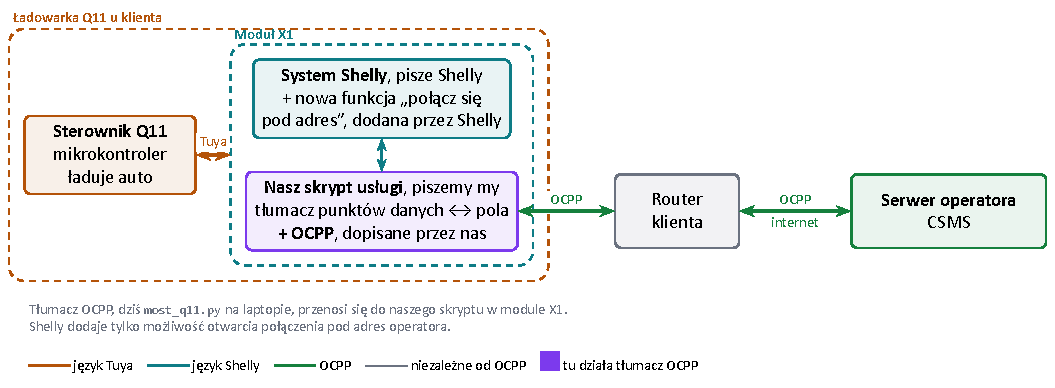
\includegraphics[width=1.00\textwidth]{img/ocpp_rozw_2_skrypt.pdf}
\caption{Rozwiązanie 2. Tłumacz przenosi się do naszego skryptu w module X1. Shelly dodaje tylko funkcję połączenia.}
\end{figure}

\subsection{W jakim module}

W tym samym module X1, który siedzi w Q11. Oprogramowanie modułu ma dwie warstwy:


\begin{itemize}
\item \textbf{System}, który pisze Shelly: Wi-Fi, szyfrowanie, połączenia, obsługa łącza z ładowarką, strona WWW, MQTT. Tej warstwy nie możemy zmienić.
\item \textbf{Skrypt usługi}, który piszemy my i wgrywamy przez portal. To nasz plik \texttt{script.\allowbreak{}svc.\allowbreak{}ts}, dziś 285 wierszy. Zamienia punkty danych Tuya na pola.
\end{itemize}

Działa to jak telefon: system pisze producent telefonu, aplikacje piszą inni. Aplikacja może tylko to, na co pozwala jej system.


\subsection{Czego dziś brakuje}

Nasz skrypt może dziś rozmawiać ze sterownikiem, ustawiać pola i odmierzać czas. W spisie funkcji modułu z 25.09 są też zapytania HTTP. Nie ma funkcji, która otwiera stałe połączenie WebSocket pod wybrany adres.


HTTP nie wystarczy. W HTTP zawsze pyta moduł, więc operator nie może sam wysłać polecenia. Moduł musiałby co chwilę pytać, czy są nowe polecenia. Przy pytaniu co 5 sekund to 17 280 zapytań na dobę z jednej ładowarki. Poza tym OCPP 1.6J z definicji działa przez WebSocket, więc serwer operatora zapytań HTTP i tak by nie przyjął.


\subsection{Jak to działa względem testu}

Shelly dodaje do systemu jedną ogólną funkcję dla skryptów: otwórz WebSocket pod adres, wyślij, odbierz. To dużo mniej pracy niż cały klient OCPP i przyda się też innym klientom Shelly. Logikę mostu, dziś 363 wiersze w Pythonie, przepisujemy na JavaScript do naszego skryptu.


\begin{longtable}{>{\raggedright\arraybackslash}p{4.93cm}>{\raggedright\arraybackslash}p{3.13cm}>{\raggedright\arraybackslash}p{7.22cm}}
\toprule
\rowcolor{apteallight}\textbf{Krok} & \textbf{Test na DevKicie} & \textbf{Rozwiązanie 2} \\
\midrule\endhead
\bottomrule\endfoot
Kto otwiera połączenie z operatorem & most na laptopie & nasz skrypt, funkcją od Shelly \\
Kto przelicza 6900 W na 10 A & most & nasz skrypt \\
Kto układa ramkę Tuya & nasz skrypt & nasz skrypt, od razu, bez przechodzenia przez pole \\
Jak poprawić błąd w OCPP & zmienić plik na laptopie & wgrać nowy skrypt przez portal; nie kasuje to ustawień Wi-Fi \\
\end{longtable}

\subsection{Czy starczy pamięci}

\leavevmode{\symbolfont\color{apamber}\textbf{◐}} To najbardziej niepewne z czterech rozwiązań. Dziś wolne jest 84 do 97 KB pamięci roboczej. Połączenie TLS zabiera przy łączeniu 40 do 50 KB, więc na skrypt z OCPP zostaje 34 do 57 KB. Skrypt działa w silniku JavaScript, a taki kod zużywa więcej pamięci niż ten sam kod wbudowany w system. Każda wiadomość OCPP to tekst, który skrypt musi rozłożyć w pamięci na części. Czy się zmieści, pokaże dopiero pomiar na module z tą funkcją.


\begin{itemize}
\item \leavevmode{\symbolfont\color{apgreen}\textbf{✔}} Bez dodatkowego sprzętu. OCPP w naszych rękach, poprawki wgrywamy przez portal.
\item \leavevmode{\symbolfont\color{apgreen}\textbf{✔}} Od Shelly potrzebna jest tylko jedna ogólna funkcja.
\item \leavevmode{\symbolfont\color{apamber}\textbf{◐}} Pamięć niepewna.
\item \leavevmode{\symbolfont\color{apred}\textbf{✘}} Nadal zależymy od Shelly, choć w mniejszym stopniu.
\item \leavevmode{\symbolfont\color{apred}\textbf{✘}} Dużo naszej pracy: przepisanie mostu i testy OCPP w JavaScript.
\end{itemize}

\clearpage
\section{Rozwiązanie 3: tłumacz na serwerze AmperePoint}

\begin{figure}[h]\centering
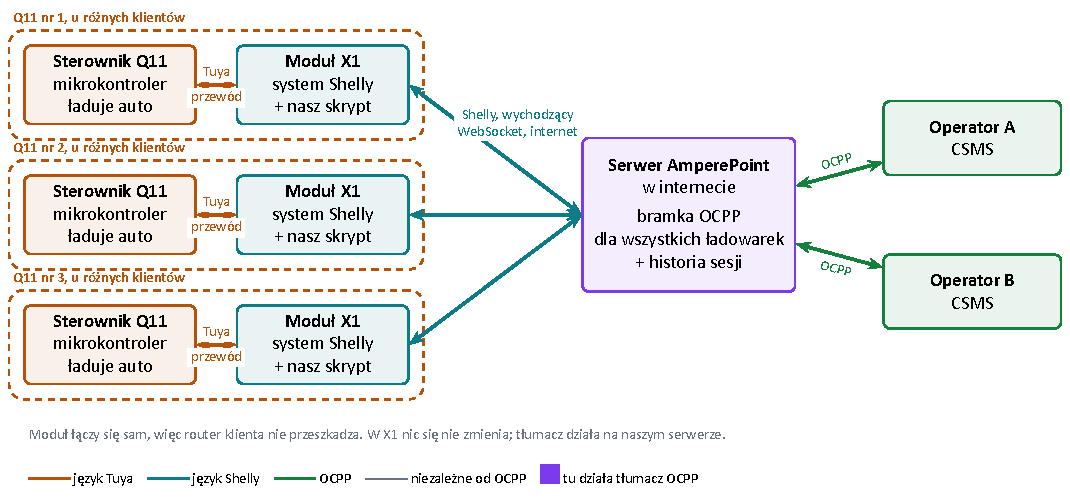
\includegraphics[width=1.00\textwidth]{img/ocpp_rozw_3_serwer.pdf}
\caption{Rozwiązanie 3. Moduły łączą się z serwerem AmperePoint, a on rozmawia z operatorami.}
\end{figure}

\subsection{Jak to działa względem testu}

To nasz most z testu, tylko przeniesiony z laptopa na serwer w internecie i obsługujący wiele ładowarek naraz.


\begin{itemize}
\item Każdy moduł X1 sam łączy się z serwerem AmperePoint i rozmawia z nim językiem Shelly, tak jak w teście DevKit z mostem. Połączenie jest wychodzące, więc router klienta go przepuszcza.
\item Moduł ma to już w systemie. W ustawieniach DevKitu z 25.09 jest pole wychodzącego WebSocketu: wyłączone, adres pusty. Nie próbowaliśmy go jeszcze włączyć. Druga droga, sprawdzona w teście, to MQTT do brokera, w internecie z TLS i hasłem.
\item Na serwerze dla każdej Q11 działa osobny tłumacz. Łączy się z operatorem tej ładowarki pod jej identyfikatorem, np. \texttt{Q11-\allowbreak{}543204516334}. Operator widzi zwykłą ładowarkę OCPP i nie musi wiedzieć o pośredniku.
\item Różne Q11 mogą mieć różnych operatorów. Serwer trzyma dla każdej adres, identyfikator i hasło.
\end{itemize}

Przykład 10 A: operator wysyła \texttt{SetChargingProfile} z limitem 6900 W do serwera AmperePoint. Tłumacz przelicza to na 10 A i wysyła polecenie Shelly przez połączenie, które moduł wcześniej otworzył. Dalej jest jak w teście: skrypt, ramka Tuya, sterownik.


Obciążenie serwera, przykład dla 500 ładowarek: znak życia co 60 s i pomiary co 30 s dają 3 wiadomości na minutę z jednej ładowarki, razem 25 na sekundę. Mniej więcej tyle samo przychodzi od modułów. To niewielki ruch nawet dla małego serwera.


\begin{itemize}
\item \leavevmode{\symbolfont\color{apgreen}\textbf{✔}} Nic nie trzeba od Shelly. Kod tłumacza już jest i działa w teście.
\item \leavevmode{\symbolfont\color{apgreen}\textbf{✔}} W X1 nic się nie zmienia, więc pamięć modułu nie jest zagrożona.
\item \leavevmode{\symbolfont\color{apgreen}\textbf{✔}} Poprawki robimy na serwerze, bez dotykania ładowarek. Na serwerze można też trzymać historię sesji dla klientów.
\item \leavevmode{\symbolfont\color{apred}\textbf{✘}} Musimy utrzymywać serwer całą dobę: koszt, zabezpieczenia, odpowiedzialność za dane klientów.
\item \leavevmode{\symbolfont\color{apred}\textbf{✘}} Gdy nasz serwer przestanie działać, wszystkie Q11 tracą połączenie z operatorami. Sterownik Q11 nadal ładuje sam, a aplikacja Shelly działa dalej, bo idzie inną drogą.
\end{itemize}

\clearpage
\section{Rozwiązanie 4: tłumacz na komputerze u klienta}

\begin{figure}[h]\centering
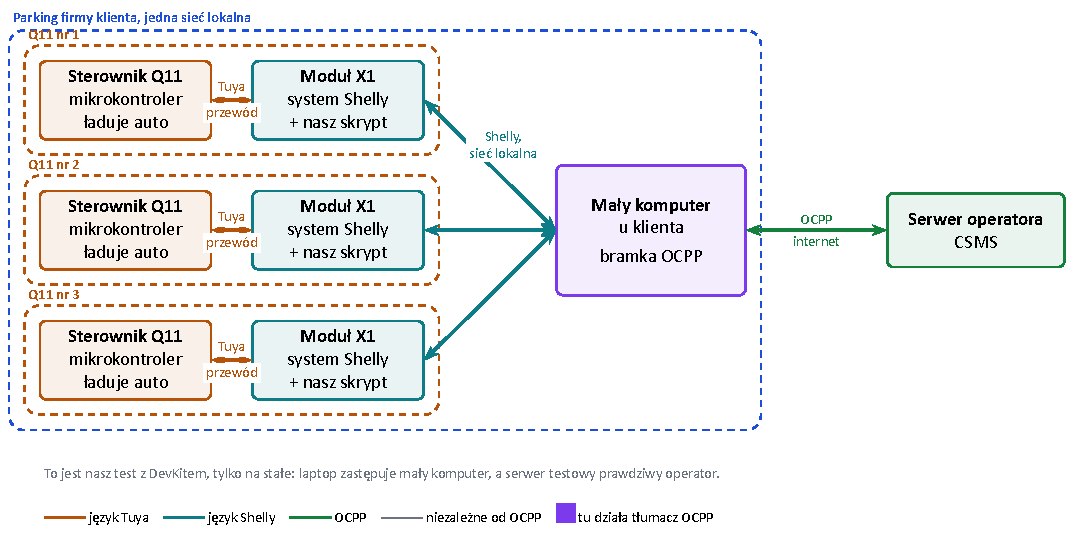
\includegraphics[width=1.00\textwidth]{img/ocpp_rozw_4_lokalnie.pdf}
\caption{Rozwiązanie 4. Mały komputer w sieci klienta obsługuje jego ładowarki.}
\end{figure}

To jest nasz test, tylko na stałe. Laptop zastępuje mały komputer, np. Raspberry Pi, który stoi w sieci klienta i działa całą dobę. Program jest ten sam, \texttt{most\_q11.py}, rozszerzony o obsługę kilku ładowarek.


Pasuje do klienta z kilkoma lub kilkunastoma Q11 w jednym miejscu, np. na parkingu firmy. Komputer może wtedy także dzielić moc przyłącza między ładowarki. Przykład: trzy Q11 po 16 A to razem 48 A na fazę, a przyłącze ma 40 A. Komputer widzi wszystkie trzy i ustawia im limity tak, by suma nie przekroczyła 40 A, również bez internetu.


\begin{itemize}
\item \leavevmode{\symbolfont\color{apgreen}\textbf{✔}} Nic nie trzeba od Shelly. Kod jest sprawdzony w teście.
\item \leavevmode{\symbolfont\color{apgreen}\textbf{✔}} Nie zależy od naszego serwera.
\item \leavevmode{\symbolfont\color{apred}\textbf{✘}} Dodatkowe urządzenie u każdego klienta: zakup, montaż, aktualizacje.
\item \leavevmode{\symbolfont\color{apred}\textbf{✘}} Przy jednej ładowarce w domu nieopłacalne.
\end{itemize}

\clearpage
\section{Porównanie}

\begin{longtable}{>{\raggedright\arraybackslash}p{3.92cm}>{\raggedright\arraybackslash}p{1.97cm}>{\raggedright\arraybackslash}p{3.01cm}>{\raggedright\arraybackslash}p{2.37cm}>{\raggedright\arraybackslash}p{3.12cm}}
\toprule
\rowcolor{apteallight}\textbf{Cecha} & \textbf{1. W systemie X1} & \textbf{2. W naszym skrypcie} & \textbf{3. Serwer AmperePoint} & \textbf{4. Komputer u klienta} \\
\midrule\endhead
\bottomrule\endfoot
Gdzie działa tłumacz & moduł X1 & moduł X1 & nasz serwer & sieć klienta \\
Kto pisze tłumacza & Shelly & my & my & my \\
Co musi zrobić Shelly & cały klient OCPP & funkcja WebSocket dla skryptu & nic & nic \\
Dodatkowy sprzęt & \leavevmode{\symbolfont\color{apgreen}\textbf{✔}} brak & \leavevmode{\symbolfont\color{apgreen}\textbf{✔}} brak & \leavevmode{\symbolfont\color{apamber}\textbf{◐}} jeden nasz serwer & \leavevmode{\symbolfont\color{apred}\textbf{✘}} komputer u każdego klienta \\
Pamięć X1 & \leavevmode{\symbolfont\color{apamber}\textbf{◐}} ciasno & \leavevmode{\symbolfont\color{apamber}\textbf{◐}} niepewne & \leavevmode{\symbolfont\color{apgreen}\textbf{✔}} bez zmian & \leavevmode{\symbolfont\color{apgreen}\textbf{✔}} bez zmian \\
Działa, gdy padnie nasz serwer & \leavevmode{\symbolfont\color{apgreen}\textbf{✔}} & \leavevmode{\symbolfont\color{apgreen}\textbf{✔}} & \leavevmode{\symbolfont\color{apred}\textbf{✘}} & \leavevmode{\symbolfont\color{apgreen}\textbf{✔}} \\
Kiedy może ruszyć & gdy zrobi to Shelly & gdy Shelly doda funkcję, plus nasza praca & od razu & od razu \\
Kto wydaje poprawki OCPP & Shelly & my, przez portal & my, na serwerze & my, na każdym komputerze \\
Co już sprawdzone & nic & nic & \leavevmode{\symbolfont\color{apamber}\textbf{◐}} logika tłumacza & \leavevmode{\symbolfont\color{apgreen}\textbf{✔}} cały łańcuch, to był nasz test \\
\end{longtable}

\section{Rekomendacja}

\textbf{Rozwiązanie 3 od razu, a Shelly zapytać o rozwiązanie 1.}


\begin{itemize}
\item Tłumacz z rozwiązania 3 już działa. W teście 25.09 przeszły rejestracja, stan, pomiary, zdalny start i limit prądu 10 A i 12 A, który Q11 potwierdziła. Trzeba go przenieść na serwer i dodać obsługę wielu ładowarek.
\item Rozwiązanie 3 nie zmienia nic w module. Pamięć robocza X1, która w rozwiązaniach 1 i 2 jest ciasna, zostaje nietknięta.
\item Rozwiązanie 1 jest najwygodniejsze dla klienta, ale zależy od Shelly. Jeśli Shelly je zrobi, Q11 można przełączyć z rozwiązania 3 na 1 zmianą ustawień w module. Operator nie zauważy różnicy, bo identyfikator ładowarki zostaje ten sam.
\item Rozwiązanie 2 zostaje planem zapasowym, gdyby Shelly odmówiło rozwiązania 1.
\item Rozwiązanie 4 ma sens tylko u klienta z wieloma ładowarkami w jednym miejscu.
\end{itemize}

\subsection{Pytania do Shelly}

\begin{enumerate}
\item Czy dodacie klienta OCPP 1.6J z TLS do systemu Shelly X? W jakim terminie i za ile?
\item Jeśli nie: czy skrypt usługi może dostać funkcję klienta WebSocket z TLS?
\item Ile pamięci roboczej zostaje dla skryptu usługi na X1 i czy starczy jej obok połączenia TLS?
\item Czy wychodzący WebSocket z ustawień modułu działa na X1 i jak serwer rozpoznaje, który moduł się połączył?
\end{enumerate}

\section{Czego jeszcze nie sprawdziliśmy}

\begin{itemize}
\item Pełnej sesji ładowania z symulatorem auta, który pobiera prąd.
\item Licznika energii. Punkt danych 1 podaje dziś 0, a operator potrzebuje stanu licznika na początku i końcu sesji do rozliczenia.
\item Wychodzącego WebSocketu modułu do serwera w internecie.
\item Połączeń z TLS i hasłem. Test był bez szyfrowania, w sieci biura.
\end{itemize}

\section*{Słowniczek}

\begin{longtable}{>{\raggedright\arraybackslash}p{2.04cm}>{\raggedright\arraybackslash}p{13.68cm}}
\toprule
\rowcolor{apteallight}\textbf{Pojęcie} & \textbf{Znaczenie} \\
\midrule\endhead
\bottomrule\endfoot
CSMS & serwer operatora, z którym łączą się ładowarki \\
OCPP 1.6J & język rozmowy ładowarki z serwerem operatora; wiadomości tekstowe JSON przez WebSocket \\
WebSocket & stałe połączenie, w którym obie strony mogą się odezwać w każdej chwili \\
HTTP & pojedyncze pytanie i odpowiedź; zaczyna zawsze pytający \\
TLS & szyfrowanie połączenia; adres zaczyna się wtedy od \texttt{wss://} zamiast \texttt{ws://} \\
Tłumacz, most, bramka & program, który po jednej stronie mówi OCPP, a po drugiej językiem Shelly \\
Język Shelly & polecenia modułu Shelly, np. „ustaw pole limitu prądu na 10” \\
Skrypt usługi & nasz program w module, wgrywany przez portal Shelly X \\
Pole & wartość w module Shelly, np. limit prądu, którą można odczytać i ustawić \\
Punkt danych & wartość w protokole Tuya, np. punkt 4 to w Q11 limit prądu \\
\end{longtable}

\section*{Źródła}

\begin{itemize}
\item Pomiary DevKitu z 25.09.2026: spis funkcji i ustawień w \texttt{DevKit\textbackslash{}logi\textbackslash{}inwentarz\_\allowbreak{}2026-\allowbreak{}09-\allowbreak{}25\_\allowbreak{}1116\textbackslash{}}, kopia pamięci flash, analiza GAP v3, rozdział 4.
\item \href{https://github.com/matth-x/MicroOcpp}{MicroOcpp, klient OCPP dla mikrokontrolerów}
\item \href{https://openchargealliance.org/ocpp-info-whitepapers/ocpp-2-lite-ocpp-for-resource-constrained-devices/}{Open Charge Alliance: OCPP dla urządzeń o małych zasobach}
\item \href{https://openchargealliance.org/wp-content/uploads/2025/03/ocpp_2_x_minimal_footprint-v14.pdf}{Open Charge Alliance: minimalne zasoby dla OCPP 2.x, PDF}
\item \href{https://docs.espressif.com/projects/esp-faq/en/latest/software-framework/protocols/mbedtls.html}{Espressif FAQ: pamięć potrzebna mbedTLS}
\item \href{https://docs.espressif.com/projects/esp-idf/en/v4.4.6/esp32/api-guides/performance/ram-usage.html}{Espressif: zużycie pamięci RAM w ESP-IDF}
\item \href{https://x.shelly.com/modules/}{Shelly X: moduły}
\end{itemize}

\end{document}